\documentclass[twocolumn,english]{article}
\usepackage[latin9]{inputenc}
\usepackage[english]{babel}
\usepackage{hyperref}
\usepackage{graphicx}

\begin{document}

\title{The SAFE Network\\ a New, Decentralised Internet [DRAFT]}
\date{October 2-3, 2014\\ Paper for the final symposium of the ADAM project}
\author{Nick Lambert\footnote{nick.lambert@maidsafe.net}\, and Benjamin Bollen\footnote{benjamin.bollen@maidsafe.net}}
\maketitle

\begin{abstract}
The Internet is an incredible resource, enabling the storage and sharing
of data amongst 40\% of the world\textquoteright s population. However,
these storage locations are inherently insecure and enable mass surveillance
and data theft by companies and world Governments. This paper proposes
a solution by redesigning and reimplementing the Internet\textquoteright s
underlying infrastructure to require no central control and by implication,
no servers as we currently know them. The ideas presented here allow
the creation of a network, which provides all users the opportunity
to retain complete control of their own security and personal information.
\end{abstract}

\section{Introduction}

Computing capability has increased dramatically in recent years, enabling
the creation of some incredible advancements. % As Moore\textquoteright s law successfully predicted for a number of years, the processing power of computers has doubled every 2 years while the increase in the connectivity of devices is growing exponentially. The so called Internet of Things (IOT - interconnection of identifiable devices), was predicted to rise from an estimated 1.3 billion devices at the end of 2010 to 1.6 billion units worldwide by the end of 2015\footnote{http://www.idate.org/en/News/Digital-Home-Connectable-devices\_693.html}.
The distribution of a faster Internet has also played its part with an estimated rise in average worldwide connection (download)
speed of 2.1Mbps in Q1 2011 to 3.9 Mbps in Q1 2014\cite{statisticaInternet14}.
These technological advancements, faster infrastructure and greater
availability have led to products and services that were previously
not possible. For example, the delivery of voice and multimedia communications
(VOIP) between mobile devices are now common place\footnote{For example, Skype usage in 2013 accounted for 214 billion minutes in 2013\cite{nay14}, or roughly 400.000 active connections on average. Since 2005 VOIP is increasingly dominating the growth of long-distance communication at the expense of conventional phone calls\cite{telegeography14}}.
These advancements have not only provided the human race with a greater
suite of tools than ever before, they have also led to fundamental
changes in how we communicate with each other. The rise of social
networking websites, mobile devices and mobile applications has led
to an explosion in what and how much data we share with each other.
%Zuckerberg\textquoteright s Law, as it has become known, takes inspiration from Moore\textquoteright s Law and states that the amount of data Facebook users share doubles every year \footnote{http://www.technologyreview.com/review/426438/the-law-of-online-sharing/}. While the maths of Zuckerberg\textquoteright s Law has been called into question by some commentators, who helpfully point out that by 2031 we will be sharing 1,048,576 times more data per day than we do at present, the sentiment that we share increasing amounts of data is clear.

This technological evolution is not only affecting how much data we
share, it is also heavily impacting upon where consumers store data.
ABI research counts 1 billion personal cloud storage accounts in 2013 with an average 685 MB stored per account.  The research forecasts a growth to 3.61 billion accounts by 2018 with an average of 975 MB per account\cite{abi13}. %This already equates over half an exabyte of personal content stored on competing cloud services.
These storage providers can be either ecosystem companies, or core cloud storage companies\footnote{Industry leaders for ecosystem providers are for example Apple, Google, Microsoft, Alibaba or Yandex. For core cloud storage companies the landscape is more dynamic, but Dropbox for personal storage or Box for business collaboration are prominent names.}, but crucially in both cases, a private company owns and controls the data, not the end-user.
%Market research agency Gartner predicts that users will store 36\% of their content online by 2016, a sharp increase from an estimated 7\% in 2011\cite{miller12}. Gartner goes on to suggest that the average household stored 464 GB online in 2011 and is forecast to rise to 3.3 TB by 2016, driven by an increased desire to share and by consumers' use of multiple devices (as storing online enables them to access all their data across all their devices).

So while these enhancements take technological ease of use to the next
level, these convenient and often free services come at a price. The
price is freedom. Today\textquoteright s centralised Internet architecture,
where centralised and managed intermediaries (servers) store and provide
access to information, do so in an inherently insecure way. We also
experience an ever increasing number of concerns over the privacy
of our data. This paper argues that it is in fact human involvement,
and the existing client server architecture\textquoteright s requirement
for human organisation, that leads to these security and privacy issues.

MaidSafe.net, a Scottish company founded for these goals, proposes and implements a new, decentralised architecture that eliminates human involvement in private data.  MaidSafe will enable users to enjoy the significant resources of the Internet, while improving and protecting their experience and privacy.


\section{The Internet is broken}

The fact that the Internet has grown beyond the expected use cases of the original design is, at the very least, a strong motivation to consider a renewed architecture. It is evident looking back that the current volume of
2.8 billion regular users\cite{mwg13} was not anticipated, nor was the original design of ARPANET centralising. In fact, one of Bob Kahn\textquoteright s fundamental rules, when designing the transmission control protocol (TCP), was that there would be no global control at the operations level\cite{isocBriefHistory}. However, some of these principles took a back seat as other considerations took priority.

It was originally envisioned, back in the late 1960s,
that there would be multiple independent networks and as Leiner et
al suggested \textquotedblleft 256 networks would be sufficient
for the foreseeable future''. This was clearly in need of consideration
when Local Area Networks (LANS) began to appear in the late 1970s. The addition of workstations, PCs and Ethernet technology, in addition to LANs, also led to changes in the original architecture
concepts. The rapid and unforeseen rise in the Internet\textquoteright s
growth introduced scaling issues\footnote{The single algorithm employed with
all routers could not cope with demand.} that were dealt with by the
implementation of a hierarchical routing model. This approach led to
a centralising of the architecture, with the introduction
of \textquotedblleft managed interconnection points\textquotedblright{}
by US Federal agencies. 

This enabled more \textquotedblleft rapid configuration robustness
and better scaling to be accommodated\textquotedblright. As the National Science Foundation (NSF) started to privatise and
commercialise the program in 1995, the use of regional networks via
private long haul carriers led to the information superhighway.  This made the world wide web, envisioned
by Tim Berners-Lee, possible. However, as the
Internet has continued to grow, it is suggested that this change in
direction has led to some significant problems that not only impact
upon the way the world\textquoteright s citizens manage data, it is also
having a much more profound impact on society as a whole. 


\subsection{Government Control}

Governments spying and eavesdropping is nothing new\cite{bbc13}. Letters have been intercepted for centuries and spy networks have existed for millennia. In recent times, attention has shifted from
telegrams to email. Within the US, Project Shamrock, established after
the Second World War, legally accessed all the cables of RCA Global,
ITT, and Western Union. Minaret was another project, established in
the 1960s to focus on intelligence gathering amongst domestic targets. Despite both programs being exposed and subsequently shelved, they
were the pre-cursor to ECHELON, a surveillance program that utilises automatic
keyword searching of faxes, telex and emails.  In 2001 the European Parliament examined the reach of the ECHELON program, but concluded the impact would be limited\cite{Schmid01}: 
\begin{quote}
[\dots] however extensive the resources and capabilities for the interception of communications may be, the extremely high volume of traffic makes exhaustive, detailed monitoring of all communications impossible in practice.
\end{quote}
 
Technological advance over the past decade has refuted the assumption of this report.  Centralisation driven by cloud services has facilitated the impact of surveillance programs. The Snowden revelations demonstrated that
intelligence agencies are able to access data at will from some of
the world\textquoteright s largest technology companies (PRISM) and
by tapping data direct from fibre optic cables (TEMPORA, FAIRVIEW,
STORMBREW, OAKSTAR and BLARNEY)\cite{guardianNSA}. Although denied by almost all technology companies, NSA slides suggest
they were complicit, willing or otherwise, in helping to collect this
data\cite{guardian13}.

This paper proposes that the existing centralised architecture and the involvement of humans, make these privacy
intrusions possible. All existing services require that users authenticate themselves.  While this process is automated, the credentials
of the users are stored in centralised locations. Furthermore, the
encryption keys are held by the service provider, enabling them to
access their user's data\cite{lambert12}. While client side encryption technology is available, it is not standard practice to implement it in end-user products. Additionally, most cloud service companies are based within the US and as such are legally obliged to comply with Government agency
requests for user data.

Interestingly, much of this monitoring conflicts with the Universal
Declaration of Human Rights that the US and UK Government and their
allies have signed up to in 1948. Article 12 states\cite{unhrd12}
\begin{quote}
\textquotedblleft No one shall be subjected to arbitrary interference
with his privacy, family, home or correspondence, nor to attacks upon
his honour and reputation. Everyone has the right to the protection
of the law against such interference or attacks.\textquotedblright
\end{quote}
The evidence suggests that, over a lengthy period, these Governments
have chosen to ignore a fundamental human right, the individual's right
to privacy. However, it is not just nations that choose to invade
our privacy.  As the Internet was designed without inherent privacy protections at protocol level, technology companies also take advantage of the centralised Internet architecture to profit from private data.

\subsection{Surveillance as a business model }

Security expert Bruce Schneier notably stated at SOURCE conference in Boston:\cite{boston14}
\begin{quote}
\textquotedblleft Surveillance is the business model of the Internet. We build systems that spy on people in exchange for services. Corporations call it marketing.\textquotedblright
\end{quote}
This suggestion is based on the fact that many large technology
companies generate the overwhelming majority of their revenue by
mining their users' data. The revenue model of companies like Google
and Facebook is to provide their core services free from monetary
charge and then sell user-targeted access to companies who advertise on their platform. Google generated USD 50.5~billion in advertising
revenue during 2013 which equated to 91\% of their yearly sales\cite{google13}. Similarly, Facebook delivered advertising revenue of over USD 6.9
billion to their investors over the same period, equivalent to 89\%
of their income\cite{facebook13}. 

Ethan Zuckerman (Director of the Center for Civic Media at MIT and
principal research scientist at MIT\textquoteright s Media Lab) has
suggested that\cite{zuckerman14}:
\begin{quote}
\textquotedblleft The fallen state of our Internet is a direct, if
unintentional, consequence of choosing advertising as the default
model to support online content and services.\textquotedblright 
\end{quote}
Zuckerman goes on to argue that Facebook, Google and others, are under
increasing pressure from shareholders to sell ever more advertisements.
They predominantly grow their advertisement revenues by providing ever deeper insights into their users.  As a result such companies mine their users' data at an ever increasing rate.

This paper suggests that the ad supported web, while not being directly
responsible for the move toward a more centralised architecture, has
nonetheless had a part to play. It is much easier to mine our data
when it is held in unencrypted and centralised locations under direct control of the service provider.

 

\subsection{Security}

Security of data is an issue that goes hand in hand with privacy,
as without security data cannot remain private. A European Commission
project, the ABC4Trust, suggests that users want privacy and organisations
want security, however, it could be argued that information stolen
from a business typically also affects individuals and therefore both
groups desire security, albeit of differing importance\cite{euABC4Trust}.

Whilst opinion on this point may vary from reader to reader, evidence
suggests that security is about as scarce as privacy within today\textquoteright s
centralised Internet. At a time when the revenue generated by the
Internet as a whole is estimated to exceed USD 4.2 trillion in G20 countries
alone, and with companies storing and sharing highly valued and sensitive
information, demand for Internet data security has never been greater\cite{bcg12}. %Previously ignored by the security community, it is now widely recognised that the weakest link in the security chain are people \footnote{http://discovery.ucl.ac.uk/144215/1/BTTJSECv5.pdf}.

In a UK Government survey on security breaches, 93\% of large organisations
and 87\% of SMEs experienced a security breach in
2013. The survey reported that major breaches were typically caused
by a combination of failures in not only people, but also process
and the technology itself\cite{ukgov13}:
\begin{quote}
\textquotedblleft 36\% of the worst security breaches in the year
were caused by inadvertent human error (and a further 10\% by deliberate
misuse of systems by staff)\textquotedblright{} 
\end{quote}
What is also evident is that these problems are not sector specific
and are taking place across all industries including healthcare, finance
and education\cite{symantec14}

With global cyber crime costing an estimated USD 400 billion per year,
it has a huge impact on society, companies and consumers\cite{mcafee14}. In December 2013, 40 million credit card details were stolen from
a prominent US retailer with the haul also including 70 million addresses
and other personal information. Similarly, in what appears to be a
series of attacks, a Russian group has amassed an estimated 1.2 billion
user names and passwords\cite{nyt14}.

With businesses continuing to store valuable information in centralised, hence inherently insecure, data centres, managed by people that empirical evidence indicates are prone to mistakes, suggests a change in approach is required. Failure
to adapt to these issues will only ensure that they continue. What is required is a change to the fundamental architecture
of the Internet; one that removes central points of weakness and humans
from the process of data management. This fresh approach should clearly
have security and privacy inherent within the design. 

%
%\section{Nature may have the answer}
%
%Complex systems have existed in nature for hundreds of millions of
%years. As the name suggests, they typically exhibit complex and often
%dynamic behaviours, that occur throughout an organisation between
%multiple component systems. These organisations are inseparable from
%their environment and continually adapt to their surroundings; examples
%include: the human brain, ant colonies, societies and the human immune
%system, to name just a few\cite{paulMS}.
%
%There are several attributes that have been identified that appear
%consistently within each Complex Adaptive System (CAS), and while
%all are important, four in particular are relevant to
%the topic of this paper, these are: distributed control; connectivity; emergent order; and a permanent state of flux.
%
%It is interesting that highly evolved natural systems self-organise with distributed control, or put another way, without centralised
%control. An iconic example of this are ant colonies, evolved over a period of 130 million years.
%
%Another important aspect of natural systems is that they remain connected,
%not only to themselves, but also to their environment. Activity within
%one part of the system ripples through and impacts upon another.
%
%Furthermore, an emergent order, defined by Chan (2001) as \textquoteleft \dots several
%agents working in parallel\textquotedblright , similar to nerve cells
%in the brain. The collective behaviour of these agents shows new behavioural features that cannot be directly explained from looking at the rules for the components alone.
%
%Such environments are highly adaptable, thriving
%on the \textquotedblleft competition and co-operation among the agents
%themselves.\textquotedblright{} As such complex systems are typically in a state of flux.
%Agents that are unable to adapt to their environment will be outcompeted. %As suggested by complex system theorists, such systems are at their most effective and productive when they are \textquotedblleft on the edge of chaos\textquotedblright \footnote{http://web.mit.edu/esd.83/www/notebook/ComplexityKD.PDF}.
%As we will see, these are attributes that are inherent within the
%proposed solution.


\section{The SAFE network; \\ a new network design}

Taking inspiration from complex natural systems, and specifically
ant colonies, Scottish engineer David Irvine set about the problem
of providing a secure data and communications platform. MaidSafe.net was founded in 2006\footnote{MaidSafe is an acronym: Massive Array of Internet Disks, Secure Access For Everyone.} to implement his design. The values of the company are to provide privacy, security and freedom for all.  The SAFE network is open source and provided free of charge to the world. %A pertinent aspect of the system design has been to decentralise online data storage while removing the need to rely on human intervention. 

The system is a fully decentralised, serverless, peer-to-peer design with
the objective of providing an autonomous global network. The network
is comprised by the users, who each donate their spare computing resources
to it and are incentivised via a network token for doing so. Each
user establishes a node, called a vault, to which the network assigns its
own unique address (derived from a cryptographic key pair). This address
is known only by the network.\cite{paulMS}

It is possible to store any type of data (structured and unstructured)
on the vault network, with typically each user running a client to enable
network requests. Vaults on the network don't
only store data, they perform multiple functions, called personas.
This includes managing the integrity of close nodes\footnote{Distance is measured with a ``bitwise exclusive or" operation on the network addresses.} and the integrity of the data chunks.  

\begin{figure}[hbtp]
\centering
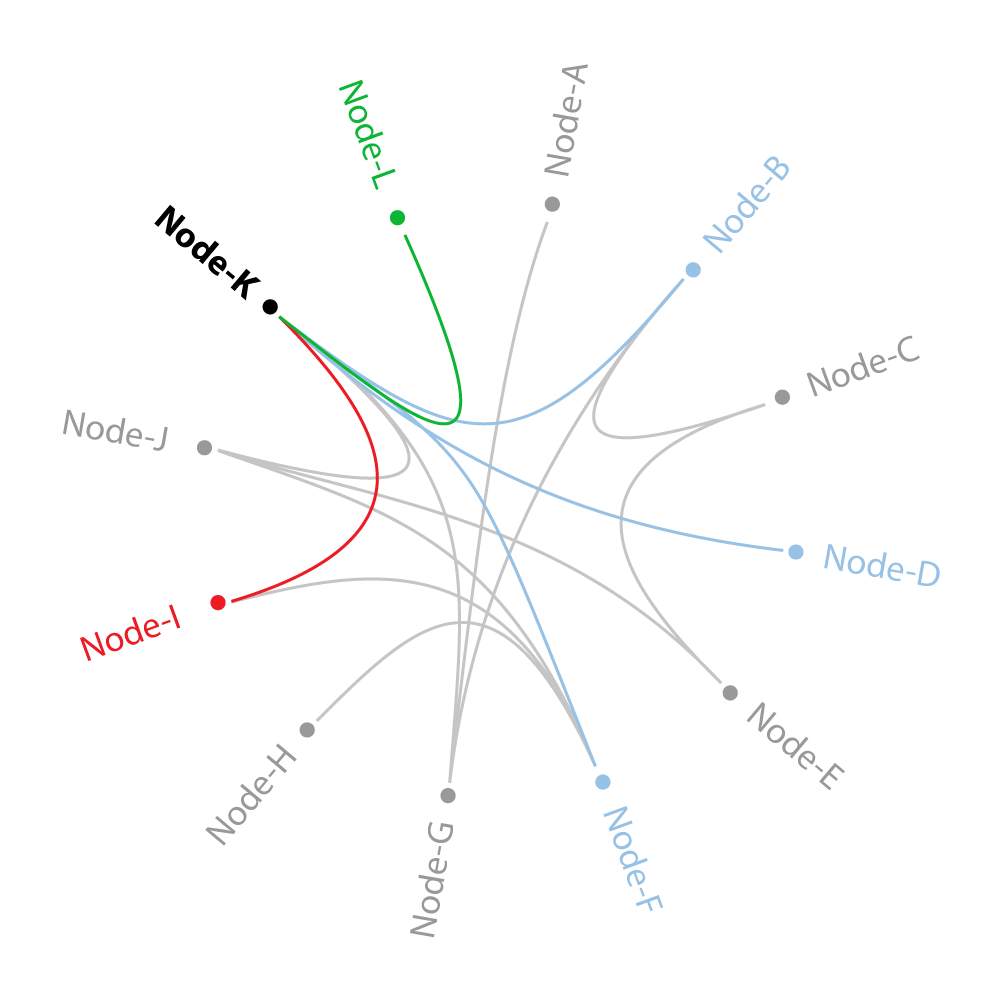
\includegraphics[scale=0.2]{connection-map.png}
\caption{Illustrative connection map of nodes showing the dynamic nature of the network. Connected lines indicate that these nodes have each other in their routing tables.  Nodes B, D, F and L are assumed to be the new close group for Node-K, where Node-I is no longer in the close group of four.}
%\vspace{1cm}
%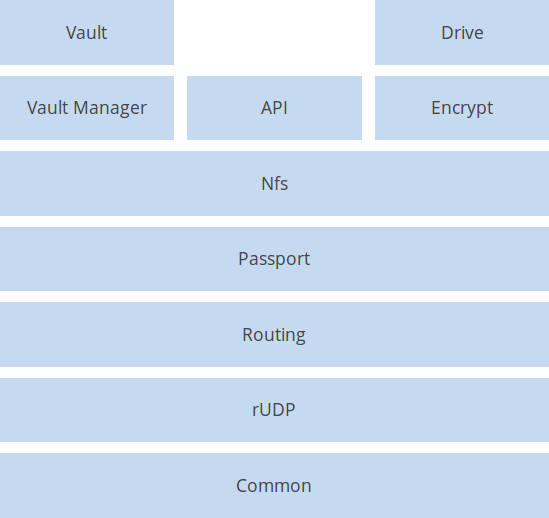
\includegraphics[scale=0.35]{stack.png}
%\caption{Diagram representing the library stack of the MaidSafe project. Refer to \ref{anatomy} Anatomy of a vault for detailed explanation.}
\end{figure}
The closest nodes will continually change as nodes go on and offline. This provides a dynamic environment.  Normal usage should  induce a high network churn. Knowledge of a network area is managed by the concept of close groups.  A close group are the vaults whose addresses closest to a given address, but not equal to it.  This determines a close group for every data chunk, but equally a close group is defined for every vault. A majority-based decision algorithm ensures that each node follows the rules of the network. It minimises undesirable or malicious behaviour, as verifiable wrong calls by a node will be monitored by its surrounding nodes.  These nodes will reduce the rank of the offending node and eventually exclude it from the network.\cite{msVault} 

Data is stored on the network in encrypted chunks. These chunks are generated by the Self-Encryption process where a sliding window encrypts and obfuscates chunks with the hash of neighbouring chunks. The final hash of the chunk serves as the name of the chunk.  This makes the network content addressable, at least when you have access to the data map to reconstruct a file\cite{msEncrypt}. Additionally this allows the network to self-heal stored data; a stored chunk whose hash does not correspond to its address has been corrupted and can be restored from redundant copies.

In the interest of data availability, the network retains minimally four live
copies of each data chunk at any time. Data managers are responsible for ensuring a new copy gets created as vaults go offline.  They also maintain a record of dead copies, as offline vaults are likely to return online later.  Because the network is content addressable, deduplication of data is utilised.

An internal study in partnership with NHS Ayrshire and Arran in 2011, showed that our algorithm achieved a 48\% deduplication rate on a 397GB data set, 312GB of which were DICOM x-ray images.

Importantly though, the MaidSafe network is the first distributed hash storage system that supports deletion of data.  The algorithm accomplishes this without explicitly listing the registered owners of chunks in the network. 


\subsection{Anatomy of a vault}\label{anatomy}

To be, or not to be written, that is the question --

\subsection{Data in a hostile environment}

The problems of data surveillance, security and privacy are multi-faceted. The SAFE network employs a range of strategies to address these problems. By decentralising the storage of data on a global network, the SAFE
network makes it more challenging for any local actor to monitor and trace information.  Data is no longer confined to a physical storage location.  Network churn makes storage a dynamical, mostly memory-to-memory operation.
As data chunks are stored with a 512bit network address and each chunk of data
is not linked to other chunks from the same file, reconstruction of a file without a datamap is both computationally infeasible and near impossible.  One needs the correct order of the correct chunks to start to decrypt AES-256.  The network will always respond to a get request; if the chunk does not exist, it will generate a random response. This largely defeats any attempt at scanning the address space.

Anonymity is a crucial element of the network. To provide a fully decentralised network, users must be able to self-authenticate onto it.  This process does not involve any register of the active users, or a third-party verification step.  Users are able to generate their own credentials and store their identity securely on the network. The credentials allow a user to retrieve a passport from the network that stores all additional keys to access and reconstruct their stored content from the network.\cite{msSA}. This provides users with the ability to manage their own
identity for the first time at network level.  The authentication process happens fully within the client computer. The password is never sent out onto the network, nor is the traffic distinguishable from other network queries.

Self-Authentication within the SAFE network provides users
with anonymity as no entity, MaidSafe included, is aware of any information
about any of the network users. Self-Authentication also ensures
that access to the network can never be restricted for any individual.

Applications on top of the SAFE network hence need to get explicit permission from any user to collect personal information.  The user can always retract these permissions and is the owner of his own data at all times.

The Self Encryption process of all data ensures that data on the network is
always encrypted, whether at rest or in transit. Data is only
ever decrypted by the client, on the end-user machine.  The encryption
password cannot be stolen from the network, as it is not given out.  

The risk remains that credentials are stolen from a compromised end-user machine.  There are measures one can take to protect against this threat, like external hardware authentication keys.  Such measures are currently beyond the scope of this article and the MaidSafe project.  As keylogging and hacking into individual end-user machines is a resource intensive tasks for any organisation, the MaidSafe network offers to level the playing field again for the opposing forces of a right to privacy and a drive for mass surveillance.

It is also worth considering the robustness that the SAFE network
provides. As the network is comprised of the resources of its users,
as opposed to a central location, it cannot be turned off and no kill
switch exists. Furthermore, the network does not use the Domain Name
System (DNS), making it impervious to web censoring. %Governments looking to stop access to the SAFE network would need to shut down access to the entire Internet to do so.

All SAFE traffic exists as fully encrypted UDP packets. This implements Net Neutrality at the core of the SAFE network.  All data packets are indistinguishable and can only be treated equally.

However, despite many of these advantages, there
are as many challenges the network needs to overcome to achieve
wide scale adoption.


\section{Discussion}

\subsection{Adoption challenges}

It is proposed that the SAFE network offers a solution to many of
the security and privacy challenges experienced with the Internet
today. However, even if the implementation and wide scale adoption
of the network is assumed, it still leaves many considerations for
which answers are not yet known. Governments will still want to surveil
both their citizens and others who they deem to be a potential threat.

As mentioned before, credentials can be stolen and human beings are often the weakest link in a security scheme.  This paper proposes that Governments may have a legitimate interest to surveil possible security threats.  However, with the introduction of the SAFE network, mass surveillance will become too resource intensive to maintain.

Attacks can also take a non-technical
form. For example, public relations efforts to discredit the network
to the public, slowing and even halting adoption are a possibility.

Removing advertising as a default form of payment for online services will
also require significant adjustment and many companies who experience success with the status quo might be resistant to
change.

However, it is important that the SAFE network does not make the advertisement driven business model impossible.  On the contrary, the SAFE network drastically cuts the infrastructure costs of online services, and a service may allow users to actively choose to pay for their usage by receiving advertisements.  The SAFE network just restores the choice to the users.

%%edit from Nick's email

Alternatively, cryptocurrencies can be part of the solution. Innovations such as Bitcoin (currently) provide very low transaction fees and can be divided with a resolution of $10^{-8}$ BTC, making micropayments a viable option. Accumulated micropayments can automatically be transferred to the correct rights holders, be it for text, music, movies or applications. At present, Bitcoin has some technical challenges regarding transaction speed\footnote{It can take up to 60 minutes to confirm a Bitcoin transaction from several miners.} that could limit its usefulness. Also the real transaction cost - disregarding mining - for a bitcoin transfer is not insignificant. This cost is volatile, but has averaged above USD 20 per transaction since December 2013\cite{blockchain14}.

The SAFE network incorporates a new cryptocurrency technology, called Safecoin.  Safecoin serves first to incentivise constructive behaviour on the network. Users are rewarded with Safecoin, paid to them by the network, as compensation for providing their computing resources. Similarly, application developers are rewarded for creating applications, based on how much their applications are used. As Safecoin transactions are not chained\footnote{Only the previous and current owner of the coin is known.} and a more efficient method of consensus is used, ie close groups within the network, it is energy-efficient and it can validate transactions at network speed. It is important Safecoin guarantees micropayments with a resolution $2^{-32}$ Safecoin. These attributes mean that it is a potentially viable way of facilitating rapid micropayments for any type of content within the network.

Clearly there is no obvious answer to the question of how to fund a new decentralised Internet, and it is out with the scope of this paper to attempt to find one. There are many alternatives and the question for users to answer is, would they rather pay for services with their freedom or with money?

%When a user choose to pay for a service, not with his privacy, but with currency, the rise of cryptocurrencies can play an important part. Currencies
%such as Bitcoin (currently) provide very low transaction fees. Accumulated micropayments can automatically be transferred to the correct rights holders, be it for text, music, movies or applications.
%At present bitcoin has some technical challenges regarding transaction
%speed that could limit its usefulness.  Also the real transaction cost (disregarding mining) for a bitcoin transfer is not small at all.
%
%The SAFE network also introduces an inherent new cryptocurrency technology, called SAFEcoin.  The initial public offering for placeholder tokens launched on April 22 2014 and was sold out in several hours.  Safecoin will be validated at network transfer speeds, and will ensure the ability to transfer micropayments.  Safecoin will be an inherent mechanism in the SAFE network to facilitate an honest quid-pro-quo strategy: you earn what you contribute to the network; and you pay for what you consume.  We look forward to the new applications developers will create with safecoin.  Safecoin is the first digital equivalent of cash money: private, instant and under your personal control.
%
%Clearly there is no obvious answer to the question of how to fund
%a new decentralised Internet, and it is out with the scope of this
%paper to attempt to find one. There are many alternatives and the
%question for users to answer is, would they rather pay for services
%with their freedom or with money?

\subsection{Competing alternatives}
[UNFINISHED, depth?]
% nice link; http://medianet.kent.edu/surveys/IAD06S-P2PArchitectures-chibuike/P2P%20App.%20Survey%20Paper.htm

MaidSafe is not the only organisation to build decentralised technologies for network infrastructure.  There are a number of alternative projects that value decentralisation. It is out with the scope of this paper to provide a detailed analysis of each.  The intention is to acknowledge that 
the SAFE network is not an isolated project. %The list is not exhaustive and restricted to decentralised technologies only.

Established in 2000, Gnutella was one of the earliest decentralised pure peer-to-peer networks and currently supports several million users.  Messages flood the network and are not [... Bens edit breaks here]

As with the SAFE network there is no
reliance on any central servers. The network is comprised of leaf nodes, nodes which have no child nodes, and ultra nodes, which are capable of routing requests and responses
from other nodes on the network.  This is accomplished via the exchange of a Query Routing Table. 
The Gnutella network has been successfully utilised by clients, such as Emule, which enable public file sharing. However, the implementation does not permit private data to be stored. 
Furthermore, data on the Gnutella network is also intended to be immutable and therefore does not enable data removal. Whilst these attributes make it well suited to public file
sharing services, it would not be a suitable replacement for all existing web services.

Freenet is another peer-to-peer network that utilises a decentralised data store that provides its users with anonymity protection and censor-resistant communications. The open source
project was established in 1999 and his been in development ever since. The network is comprised of multiple nodes, some of which act as hosts for data and others which only route the 
flow of data. Every node on the network contributes storage space and data is stored in encrypted blocks and spread on several network nodes. 
Unlike the SAFE network, which was designed as a decentralised data and communications network, Freenet was primarily designed as a network for the publication of files and is not 
intended to limit access to those files. There is no mechanism to delete data on the network, however, information that is not retrieved regularly can drop off the network as allocated disk 
space is utilised. This approach makes Freenet an effective anonymous publishing platform, but its lack of storage and management of private data limits its potential to replace the todays
existing centralised web services. 

Bittorrent is the most popular peer-to-peer networks which, according to the company, is used by an estimated 150 million users world wide.

\section*{Conclusion}

The SAFE network potentially provides a solution to those looking
to enjoy the vast resources of the Internet without many of the downsides,
which include mass surveillance from governments and companies. The SAFE
network also aims to minimise many of the security risks that currently
exist with the existing world wide web. The SAFE network has been implemented
in a decentralised architecture and has been designed in this way
to remove the requirement for human intervention from our data, while
also removing servers, which act as a central point of weakness.


\begin{thebibliography}{9}

\bibitem{statisticaInternet14} Statista, \emph{Average Global Internet Connection Speed from 1st Quarter 2011 to 1st Quarter 2014}, \href{http://www.statista.com/statistics/204954/average-internet-connection-speed-worldwide/}{statista.com 2014}

\bibitem{nay14} J.R. Nay, \emph{Skype's Worldwide Traffic Continues to Grow, with 214 Billion Minutes on VOIP in 2013}, \href{http://www.trutower.com/2014/01/13/skype-voip-app-calling-statistics-telegeography/}{TruTower, January 13, 2014}

\bibitem{telegeography14} PriMetrica, \emph{TeleGeography Report 2013}, \href{http://www.telegeography.com/page_attachments/products/website/research-services/telegeography-report-database/0004/6341/TG_executive_summary.pdf}{Executive Summary}

%\bibitem{miller12} C. Miller, \emph{Gartner: Consumers Will Drive Huge Growth for Cloud Storage}, \href{http://www.datacenterknowledge.com/archives/2012/07/02/gartner-consumers-will-store-more-in-the-cloud}{Data Center Knowledge, July 2, 2012}

\bibitem{abi13} ABI Cloud Content and Services Research service, \emph{Personal Cloud Storage and Synchronization Study}, \href{https://www.abiresearch.com/press/personal-cloud-storage-accounts-total-one-billion-}{Personal Cloud Storage Accounts Total One Billion in 2013, Generating 685 Petabytes, Research News December 13, 2013}

\bibitem{mwg13} Internet World Stats, \emph{Internet Users in the World Q4 2013}, \href{http://www.internetworldstats.com/stats.htm}{Miniwatts Marketing Group Internet World Stats}

\bibitem{isocBriefHistory} V. Cerf et al, \emph{Brief History of the Internet}, \href{http://www.internetsociety.org/internet/what-internet/history-internet/brief-history-internet}{Internet Society}

\bibitem{bbc13} A. Zurcher, \emph{Roman Empire to the NSA: A World History of Government Spying}, \href{http://www.bbc.co.uk/news/magazine-24749166}{BBC News, November 1, 2013}

\bibitem{Schmid01} G. Schmid, \emph{On the existence of a global system for the interception of private and commercial communications (ECHELON interception system)}, \href{http://www.europarl.europa.eu/sides/getDoc.do?pubRef=-//EP//TEXT+REPORT+A5-2001-0264+0+DOC+XML+V0//EN}{European Parliament report PE 305.391, A5-0264/2001, July 2001}

\bibitem{guardianNSA} The Guardian, \emph{The NSA Files}, \href{http://www.theguardian.com/world/the-nsa-files}{www.theguardian.com/world/the-nsa-files}

\bibitem{guardian13} G. Greenwald and E. MacASkill, \emph{NSA Prism program taps in to user data of Apple, Google and others}, \href{http://www.theguardian.com/world/2013/jun/06/us-tech-giants-nsa-data}{The Guardian, June 7 2013}

\bibitem{lambert12} P. Lambert, \emph{Does your cloud storage provider hold the keys to your data}, \href{http://www.techrepublic.com/blog/it-security/does-your-cloud-storage-provider-hold-the-keys-to-your-data}{TechRepublic.com, April 9, 2012}

\bibitem{unhrd12} United Nations General Assembly, \emph{The Universal Declaration of Human Rights}, \href{http://www.un.org/en/documents/udhr/}{Human Rights Declaration, article 12, December 10, 1948}

\bibitem{boston14} SOURCE conference Boston 14, \emph{keynote speech} by Bruce Schneier, \href{http://sourceconference.com/boston/}{Boston, April 2014}; F.Y. Rashid \emph{Surveillance is the Business Model of the Internet: Bruce Schneier}, \href{http://www.securityweek.com/surveillance-business-model-internet-bruce-schneier}{Security Week April 9, 2014}

\bibitem{google13} Google Investor Relations, \emph{Google's Income Statement Information}, \href{https://investor.google.com/financial/2013/tables.html}{Financial Tables 2013}

\bibitem{facebook13} Facebook Investor Relations, \emph{Facebook reports Fourth Quarter and Full Year 2013 Results}, \href{http://investor.fb.com/releasedetail.cfm?ReleaseID=821954}{Fourth Quarter and Full Year 2013 Financial Summary}

\bibitem{zuckerman14} E. Zuckerman, \emph{The Internet's Original Sin}, \href{http://www.theatlantic.com/technology/archive/2014/08/advertising-is-the-internets-original-sin/376041/}{The Atlantic, August 14, 2014}

\bibitem{euABC4Trust} European Commission, \emph{Security and privacy? Now they can go hand in hand}, \href{https://ec.europa.eu/digital-agenda/en/news/security-and-privacy-now-they-can-go-hand-hand}{Digital Agenda for Europe, News, May 27, 2014}

\bibitem{bcg12} The Boston Consulting Group, \emph{The Internet Economy in the G-20}, \href{https://www.bcg.com/documents/file100409.pdf}{BCG report, the connected world, the internet economy in the G-20, March 2012}

\bibitem{ukgov13} Department for Business Innovation and Skills, UK government, \emph{2013 Information Security Breaches Survey}, \href{https://www.gov.uk/government/uploads/system/uploads/attachment_data/file/191671/bis-13-p184es-2013-information-security-breaches-survey-executive-summary.pdf}{Executive Summary BIS/13/P184 - ES, technical report 2013}

\bibitem{symantec14} Symantec, \emph{In Defense of Data}, \href{http://www.symantec.com/connect/blogs/data-breach-trends}{Symantec Official Blog, January 1, 2014}

\bibitem{mcafee14} McAfee, \emph{Stopping Cybercrime Can Positively Impact World Economies}, \href{http://www.mcafee.com/uk/about/news/2014/q2/20140609-01.aspx}{McAfee Press Release June 9, 2014}

\bibitem{nyt14} N. Perlroth and D. Gelles, \emph{Russian Hackers Amass Over a Billion Internet Passwords}, \href{http://www.nytimes.com/2014/08/06/technology/russian-gang-said-to-amass-more-than-a-billion-stolen-internet-credentials.html}{New York Times August 5, 2014}

\bibitem{paulMS} G. Paul, F. Hutchison, J.Irvine, \emph{Security of the MaidSafe Vault Network}, \href{https://pure.strath.ac.uk/portal/files/34898763/Paul_etal_wwrf32_vault_network.pdf}{in collaboration with University of Strathclyde}

\bibitem{msVault} MaidSafe, \emph{Vault Documentation}, \href{https://github.com/maidsafe/MaidSafe-Vault/wiki/Documentation}{GitHub MaidSafe-Vault documentation}

\bibitem{msEncrypt} MaidSafe, \emph{MaidSafe Encrypt Library}, \href{http://maidsafe.net/libraries-encrypt}{MaidSafe-Encrypt overview}

\bibitem{msSA} MaidSafe, \emph{MaidSafe Self-Authentication}, \href{http://maidsafe.net/Whitepapers/pdf/SelfAuthentication.pdf}{MaidSafe Self-Authentication paper, September 2010}

\bibitem{blockchain14} Blockchain, \emph{Cost per Transaction}, \href{https://blockchain.info/charts/cost-per-transaction}{chart produced by blockchain.info, time of writing September 2014}

\end{thebibliography}
\end{document}
